\chapter{Introduction}

  This chapter explains the two basic notions fundamental to the ideas developed in this thesis. Firstly,
  \keyword{sparse banded matrices derived from structured grids}, their usage in the natural sciences and their
  particular structure are introduced and, secondly, the general purpose \keyword{compressed sparse row matrix storage
  format} (CSR) used for sparse matrix arithmetic.

  \section{Sparse Banded Matrices Derived from Structured Grids} \label{sec:structured-grid-matrices}

    Structured grid computations are ubiquitously used for physical simulations in scientific fields such as, for
    example, computational fluid dynamics, electrodynamics and astrophysics. Generally, a system of partial differential
    equations is solved by discretization and linearization of the problem which involves generating a grid
    corresponding to the physical domain in question. A structured grid refers to a mesh whose nodes are uniquely
    identified by a tuple of coordinates and v.v., such as $(i, j, k)$ for three dimensions (Figure
    \ref{fig:structured_grid_example}). Such meshes are sometimes referred to as \emph{logically rectangular}.

    \begin{figure}[ht]
        \centering
        \vspace{0.5cm}
        \begin{minipage}{0.4\textwidth}
          \centering
          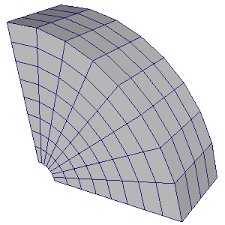
\includegraphics[width=0.9\textwidth]{fig/structured_grid_example.png} % second figure itself
          \toccaption{Curvi-linear grid over a physically complex domain.}{ The grid nodes are logically rectangular
            despite the non-rectangular physical domain and thus comprise a structured grid. Source:
            \cite{daad:website}}
          \label{fig:structured_grid_example}
        \end{minipage}\hfill
        \begin{minipage}{0.5\textwidth}
          \centering
          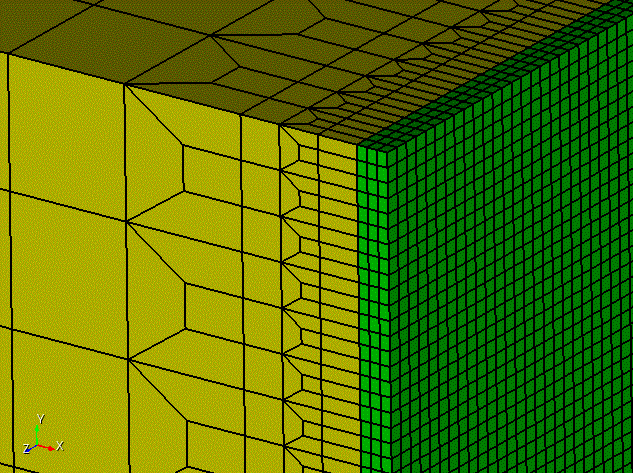
\includegraphics[width=0.9\textwidth]{fig/refined_structured_grid.png} % second figure itself
          \toccaption{Heterogeneous mesh with structured regions.}{Outer side (green) and interior volume are fully
            structured and are connected via an unstructured mesh region. Given proper indexing of grid nodes the
            resulting sparse matrix will exhibit regularity in the sections pertaining to the structured mesh region.
            Source: \cite{cubit-mesh-refinement:website}}
          \label{fig:refined_structured_grid}
        \end{minipage}
    \end{figure}

    In contrast to unstructured grids the regularity inherent to structured grids allows for very efficient numerical
    treatment, such that even in cases where sufficiently complex geometries prohibit the decomposition of the target
    domain into a single overarching structured grid the domain is often tesselated into an unstructured configuration,
    with the tiles being filled by independent structured grids \cite{Badcock2000}(Figure
    \ref{fig:refined_structured_grid}).

    \begin{figure}
        \centering
        \captionsetup{width=0.9\columnwidth}
        \begin{minipage}{0.45\textwidth}
          \centering
          \begin{tikzpicture}[scale=0.65]%[every node/.style={minimum size=1cm},on grid]
\newcommand*{\height}{5}
\newcommand*{\width}{5}
\begin{scope}[every node/.append style={yslant=-0.5},yslant=-0.5]
  \shade[right color=gray!10, left color=black!50] (0,0) rectangle +(\width,\height);

  \foreach \x in {1,...,\width}
    \foreach \y in {1,...,\height}
    {
        \node at (-0.5 + \x, -0.5 + \y) {\pgfmathtruncatemacro\result{21-5*(\x-1)+25*(\y-1)}$\result$};
    }
  \draw (0,0) grid (\height,\width);
\end{scope}
\begin{scope}[every node/.append style={yslant=0.5},yslant=0.5]
  \shade[right color=gray!70,left color=gray!10] (\width,-\height) rectangle +(\height,\width);
    \foreach \x in {1,...,\width}
    \foreach \y in {1,...,\height}
    {
        \node at (\width - 0.5 + \x, -\height + -0.5 + \y) {\pgfmathtruncatemacro\result{1 + 1*(\x-1)+25*(\y-1)}$\result$};
    }

  \draw (\width,-\height) grid (2*\width,0);
\end{scope}
\begin{scope}[every node/.append style={
    yslant=0.5,xslant=-1},yslant=0.5,xslant=-1
  ]
  \shade[bottom color=gray!10, top color=black!80] (2*\width,\height) rectangle +(-\width,-\height);

    \foreach \x in {1,...,\width}
    \foreach \y in {1,...,\height}
    {
        \node at (\width - 0.5 + \x, -0.5 + \y) {\pgfmathtruncatemacro\result{101 + 1*(\x-1)+5*(\y-1)}$\result$};
    }

  \draw (\width,0) grid (2*\width,\height);
\end{scope}
\end{tikzpicture}

        \end{minipage}
        \begin{minipage}{0.45\textwidth}
            \centering
            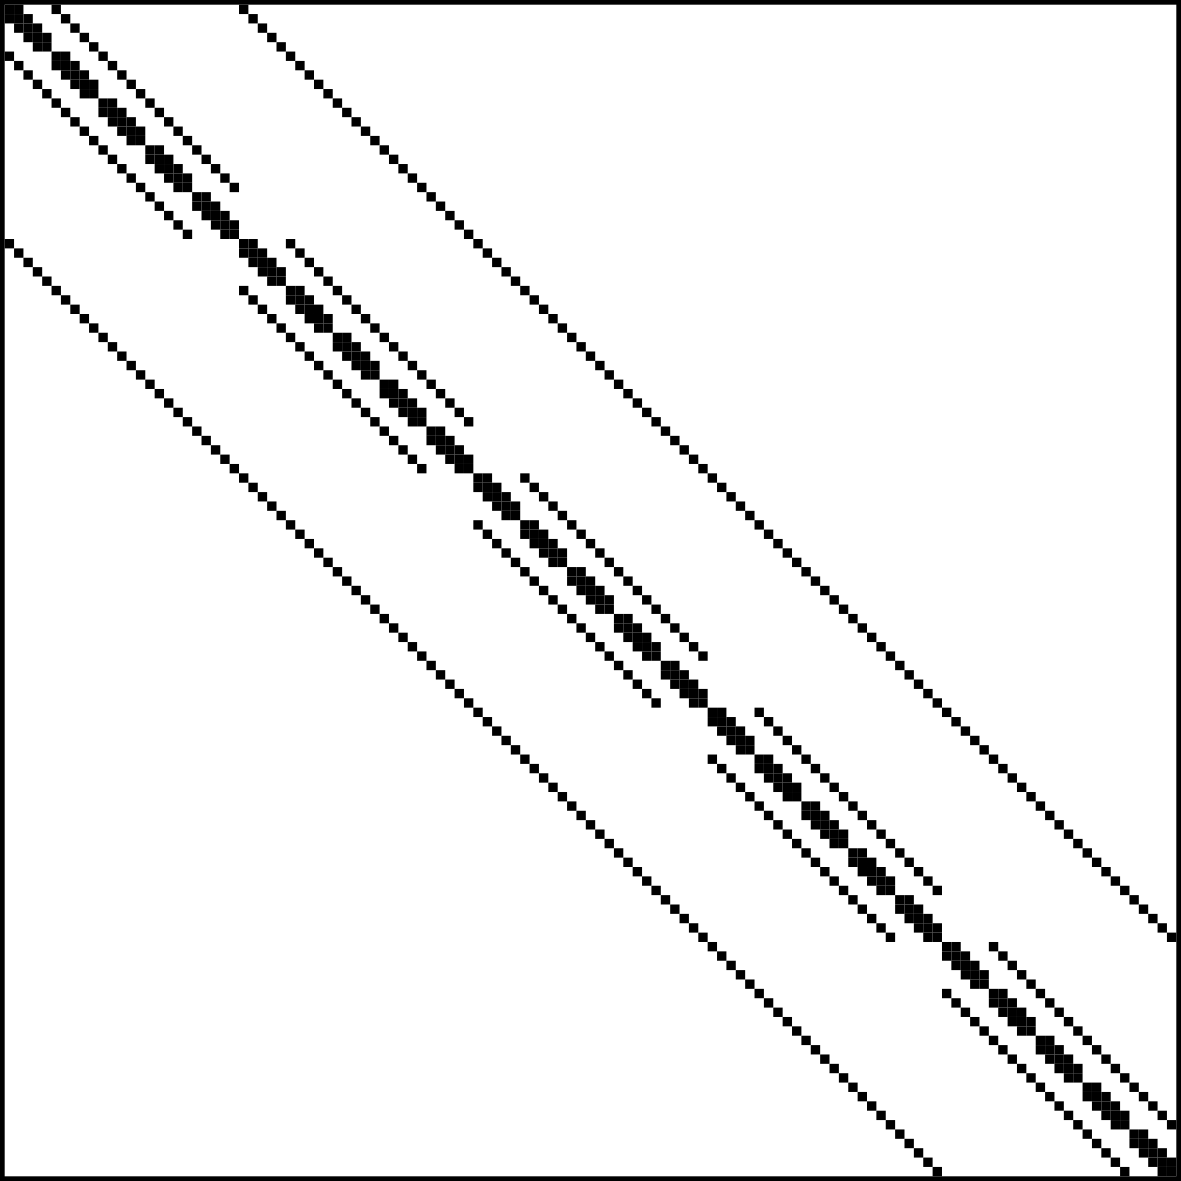
\includegraphics[width=0.9\textwidth]{fig/laplacian_example.png} % second figure itself
        \end{minipage}
        \toccaption{Structured grid and corresponding matrix for a simple Laplacian.}{Structured grid and corresponding
          matrix for a simple Laplacian $\nabla^2 u(\vec{r}) = 0$. The Laplace-operator is approximated by the
          conventional 3-axial symmetric discretization scheme, equivalent to a symmetric 7-point stencil operation.}
        \label{fig:laplacian-example}
    \end{figure}

    The solution procedure yields a sparse linear system whose solution is approximated by iterative methods involving
    repeated sparse matrix-vector-multiplications $Ax = b$ where the matrix $A$ encodes the adjacency structure of the
    grid. For a structured grid, the resulting matrix's distribution of non-zeros has a very distinct pattern. Generally
    speaking, such matrices consist of multiple diagonals of non-zero values at fixed intervals while all other elements
    are zero. The diagonals are almost fully dense with exceptions arising at positions corresponding to nodes at the
    grid's boundaries, where the regular adjacency pattern of the grid is disturbed by missing nodes. A grid and its
    corresponding sparse matrix's structure are depicted in Figure \ref{fig:laplacian-example} for a simple Laplacian
    problem.

    The matrix's non-zero values depend on the underlying physical problem's parameters, the type of PDE and the
    differential operators' discretization schemes. In general, the non-zeros' numeric values are independent of their
    location within the matrix but there exist classes of problems where the presence of a matrix slice whose rows
    have diagonal structure implies that those rows share the same numeric values. Furthermore, solving problems on
    multiple coupled entities such as vectors or matrices yields sparse banded matrices whose 'elements' are themselves
    square matrices \cite{Godwin2013}.

    The sparse matrices relevant to this work are any sparse matrices that contain one or more sets of rows whose
    non-zero's column indices share the same values save for a fixed offset. Sparse banded matrices arising from the
    procedure mentioned above have one such set to which the overwhelming majority of rows belong corresponding to all
    inner grid nodes (such as in the example in Figure \ref{fig:laplacian-example}). Such matrices shall be referred to
    as sparse banded matrices derived from structured grids for the purpose of this text. However, all of the ideas
    presented hereinafter may be applied to any sparse matrix whose structure exhibits any degree of repetitiveness.

  \section{Compressed Sparse Row Matrix Storage Format}

    The compressed sparse row (CSR) format is a widely used storage format for sparse matrices. Unlike other popular
    sparse matrix storage formats such as the diagonal storage format (DIA), the CSR format is not tailored to any
    special type of matrix but is a general purpose storage format that makes no assumptions about the matrix's shape or
    its distribution of non-zeros. The CSR format can be considered an improvement to the naive coordinate format (COO)
    in that each non-zero's row index is no longer explicitly stored \cite{Bell2011}.

    The CSR format consists of three dense arrays. The values array (V) stores the numerical value for each non-zero
    entry in the matrix while the associated column index is stored in the column-index array (CI). A third array, the
    row-pointer array (RP), encodes the beginning of each row's section within the values and column-index arrays, i.e.
    it stores the offset of each row's first non-zero element into the two arrays. By convention, the row-pointer array
    usually also contains an additional element denoting the total number of non-zero elements in the matrix. An example
    for the CSR format is given in Figure \ref{fig:csr_example}.

    \begin{figure}[ht]
      \centering
      \captionsetup{width=0.9\columnwidth}
      \begin{minipage}{0.4\textwidth}
        \centering
        $$
        \begin{pmatrix}
          \color{red}{\bm{3}} &                     0 &  \color{red}{\bm{4}} &                    0 \\
                            0 & \color{green}{\bm{1}} &                    0 &                    0 \\
                            0 &                     0 & \color{blue}{\bm{7}} & \color{blue}{\bm{8}} \\
        \end{pmatrix}
        $$
      \end{minipage}
      \begin{minipage}{0.4\textwidth}
        \centering
        $$
        \begin{matrix}
          \text{Values}  & : & \color{red}{3} &   \color{red}{4} & \color{green}{1} & \color{blue}{7} & \color{blue}{8} \\
          \text{Column-Indices} & : & \color{red}{0} &   \color{red}{2} & \color{green}{1} & \color{blue}{2} & \color{blue}{3} \\
          \text{Row-Pointers} & : & \color{red}{0} & \color{green}{2} &  \color{blue}{3} &               5 &                 \\
        \end{matrix}
        $$
      \end{minipage}
      \toccaption{Exemplary matrix with corresponding CSR representation.}{The array elements are color-coded in red for
        the first row, green for the second row and blue for the third row.}
      \label{fig:csr_example}
    \end{figure}

    Thus, as previously mentioned, the CSR format optimizes the storage requirements of general sparse matrices with
    respect to the naive coordinate format (COO) shrinking the size of the third array from one entry per non-zero
    element to a single entry per row irrespective of the row's number of non-zeros. Furthermore, the existing
    literature, in part, utilizes a different nomenclature referring to the arrays as A (values array), JA (column-index
    array) and IA (row-pointer array), respectively \cite{sparskit}.

    The CSR format's salient feature is the contiguousness of the rows' non-zero elements' values and column indices
    making it particularly well suited for matrix-vector-multiplication utilizing a conventional row-by-column
    computation scheme due to ideal data locality for the values and column arrays, although accesses into the argument
    vector during multiplication are suboptimal. Aside of this characteristic storing the non-zero elements row-by-row
    as opposed to column-by-column is a choice and thus some numerical libraries and toolkits such as the Eigen C++
    library \cite{eigen:website} or the Harwell-Boeing sparse matrix collection \cite{harwell-boeing} utilize the
    CSR format's conjugate, the compressed sparse column format (CSC), as their default means of storing sparse
    matrices.

    The CSR format serves as a starting point for the C3SR sparse matrix storage format for sparse banded matrices which
    is the focal point of this work.

